\documentclass[dvisvgm]{standalone}

\usepackage{tikz}
\usetikzlibrary {arrows, positioning, automata}

\begin{document}

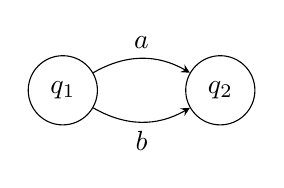
\begin{tikzpicture}[
    ->,
    >=stealth,
    node distance=2cm,
    initial text=$ $,
    on grid,
]

    \node[           state]              (A) {$q_1$};
    \node[           state, right =of A] (B) {$q_2$};

    \path
        (A) edge [above, bend left]       node {$a$}  (B)
        (A) edge [below, bend right]      node {$b$}  (B)
    ;
\end{tikzpicture}

\end{document}